\chapter{Spektren}
Wir haben bisher zwei Beschreibungsebenen für diskrete Signale und
Systeme kennen gelernt, den Zeitbereich mit der
Differenzengleichung und die z-Ebene. Häufig ist aber von
Interesse, wie sich die Signale und Systeme in Abhängigkeit von
der Frequenz verhalten. Diese Darstellung wird als Spektrum
bezeichnet. Dabei ist das Betragsverhalten (Betragsspektrum), also
ob und mit welcher Leistung eine Frequenz im Signal vorhanden ist
oder ob ein System eine bestimmte Frequenz verstärkt oder dämpft,
interessant. Das Phasenverhalten ist für viele Anwendungen von
sekundärer Bedeutung. Trotzdem kann insbesondere bei der
Beschreibung von Systemen das Phasenspektrum eine wichtige
Information darstellen.

\tbd{Motivationsbeispiel: Feedbackproblematik im Hörgerät oder bei
der Bühnenbeschallung. Analyse des Signals (Spektrum) ermöglicht
zu erkennen, bei welcher Frequenz die Störung auftritt. Nach der
Analyse kann bei dieser Frequenz ein System eingebaut werden, dass
die Übertragung dämpft. Durch den frequenzselektiven Eingriff wird
das Nutzssignal nur unwesentlich beeinflusst.}

\tbd{Aktives Beispiel wäre schön.}

Eine Möglichkeit das Verhalten bei einer bestimmten Frequenz zu
testen, ist, das LTI-System mit Signalen anzuregen die nur aus
einer Frequenz bestehen und dann die Veränderung am Ausgang zu
messen. Ein sehr gutes Eingangssignal um Betrag und Phase zu
bestimmen ist die ungedämpfte diskrete Exponentialschwingung
\begin{equation}\label{eq:Def:Euler}
    e^{j\Omega_0 k} = \cos(\Omega k)+j\sin(\Omega k)
\end{equation}
mit $\Omega_0 = 2 \pi f_0/ f_s$, wobei $f_0$ die Analysefrequenz und
$f_s$ die Samplingfrequenz angibt.

\hspace{1cm}\begin{minipage}{10cm}
{\bf Exkurs: Frequenzachsen in der DSV}
Manchmal ist es verwirrend in welcher Form Frequenzen in der
digitalen Signalverarbeitung angegeben werden. Die am häufigsten verwendeten Systeme
und ihre Äquivalenz als Achse und ihre Position auf dem Einheitskreis in der z-Ebene zeigt
Abbildung \ref{pic:FrequenzenDSV}.
\begin{figure}[H]
\begin{center}
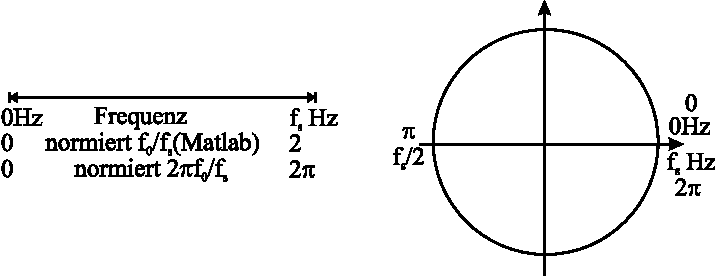
\includegraphics{psSpek/FrequenzskalierungenExkurs}
\caption{\label{pic:FrequenzenDSV}Veranschaulichung der unterschiedlichen Frequenzbezeichnungen
in der DSV und ihre Position auf dem Einheitskreis in der z-Ebene.}
\end{center}
\end{figure}
\end{minipage}

Mit Hilfe der Faltung ergibt sich am Ausgang eines durch die
Impulsantwort beschriebenen Systems.
\begin{eqnarray}\label{eq:fTrafo:Bsp}
    y(k)& = &x(k)\ast h(k) = \sum_{\kappa = -\infty}^{\infty} h(\kappa)
    e^{j\Omega_0(k-\kappa)}\\
    &= & \underbrace{e^{j\Omega_0 k}}_{\mbox{Eingangssignal}} \cdot
    \underbrace{\sum_{\kappa = -\infty}^{\infty} h(\kappa) e^{-j\Omega_0
    \kappa}}_{\mbox{Komplexer Multiplikator}}
\end{eqnarray}
Das heißt also, am Ausgang können wir eine Schwingung derselben
Frequenz messen, die nur in ihrer Phase und ihrem Betrag geändert
wird. Berechnen wir dieses Ausgangsverhalten für alle Frequenzen
erhalten wir das Spektrum. Auffällig bei LTI-Systemen ist, das
keine neuen Frequenzen entstehen. Dies ist eine typische
Eigenschaft von LTI-Systemen.

\wichtig{LTI-Systeme erzeugen keine neuen Frequenzen}

Bei Systemen wird die frequenzabhängige Veränderung des Betrages
und der Phase Übertragungsfunktion genannt und kann mit
\begin{equation}\label{eq:DTFD:Hin}
    H \jom = \sum_{k = -\infty}^{\infty} h(k) e^{-j\Omega k}
\end{equation}
berechnet werden. Diese Form ist eng verwandt mit der
Fourier-Transformation für analoge Signale und wird deshalb
Zeitdiskrete Fourier-Transformation ({\em Discrete Time
Fourier-Transformation (DTFT)}) genannt.

Vergleichen wir nun Gleichung \ref{eq:DTFD:Hin} mit der Definition
der z-Transformation, so erkennen wir, dass die DTFT die
z-Transformation für $z = e^{j\Omega}$ darstellt und somit genau
den Einheitskreis in der z-Ebene beschreibt. Wir können also
direkt am Einheitskreis das frequenzabhängige
Übertragungsverhalten von Systemen ablesen. Dies gilt analog
natürlich auch für Signale.

Kennen wir also die z-Transformation eines Systems können wir auch
sofort die Übertragungsfunktion angeben. Betrachten wir
beispielsweise das System $y(k) = x(k) + x(k-1)$, dann ergibt
$e^{j\Omega}$ in die z-Transformierte eingesetzt
\begin{equation}\label{eq:fTRafo:Bsp:zTrafoFTrafo}
    H \jom = 1+z^{-1} \Big|_{z = e^{j\Omega}} = 1+e^{-j\Omega}
\end{equation}
Durch Umformungen erhalten wir.
\begin{eqnarray}\label{eq:fTrafo:BspUebrtragungF}
   e^{j\Omega / 2} H \jom &= & e^{j \Omega / 2}+e^{-j\Omega / 2}\\
   & = & \underbrace{2 \cos(\Omega / 2)}_{\mbox{Betrag, wenn $|\cdot|$}}
   \underbrace{e^{-j\Omega / 2}}_{\mbox{Phase}}
\end{eqnarray}

Die komplexwertige Darstellung mit Real und Imaginärteil ist dabei
zur Veranschaulichung und Interpretation nicht geeignet. Statt
dessen wird das komplexe Signal meist in den Betragsfrequenzgang,
d.h, eine Darstellung von $|H \jom|$ über der Frequenz und den
Phasengang, eine Darstellung des Arguments von $H \jom$,
aufgeteilt, wobei beim Betrag oder dem Betragsquadrat auch häufig
eine logarithmische Darstellung gewählt wird

\section{Einfluss der Pole und Nullstellen auf die Übertragungsfunktion}
Um den Einfluss der Pole und Nullstellen auf die
Übertragungsfunktion abzuschätzen, schauen wir uns zunächst noch
einmal die Abbildung \ref{pic:PolNullstellenAuswirkung} an. Bei
dieser Abbildung ist $|H \jom|^2$ logarithmisch dargestellt. Der
Betragsfrequenzgang der DTFT kann direkt aus dem enstehenden
''Gebirge'' abgelesen werden, wenn wir den Einheitskreis vom
Winkel $0$ bis $\pi$ umlaufen. Der Pol bei $\pi/10$ verursacht
eine Verstärkung auf dem Einheitskreis. Ein Pol direkt auf dem
Einheitskreis würde zu einer unendlichen Verstärkung führen.
Sobald der Winkel größer wird als $\pi/10$ nimmt die Verstärkung
ab. Ab einem Winkel von $\pi/2$ werden die Nullstellen dominant,
die dazu führen, dass sich der Betragsfrequenzgang null nähert und
die Null bei genau $\pi$ erreicht. Auf dem unteren Halbkreis geht
zunächst der Einfluss der Nullstelle zurück und der konjugiert
komplexe Pol bei $-\pi/10$ gewinnt an Einfluss. Bei $\Omega =
2\pi$ sind wir erneut bei $\Omega = 0$. Der Betragsfrequenzgang
wiederholt sich also periodisch in $2\pi$ für diskrete Signale.
Dies ist auch direkt aus der Beziehung
\begin{equation}\label{Eq:Spek:PeridozitaetsERklaerung}
    e^{j\Omega k} = e^{j(\Omega +2\pi n) k} \quad \forall \quad n \in \mathbb{N}
\end{equation}
zu sehen.

Eine direkte Berechnung des Betrag- und Phasenganges aus den Polen
und Nullstellen ist ebenfalls möglich. Um das zu veranschaulichen
ist in Abbildung \ref{pic:SpecPolNullstellen} ein System zweiter
Ordnung in der z-Ebene mit den zwei Polen und den zwei Nullstellen
gezeigt.
\begin{figure}[H]
\begin{center}
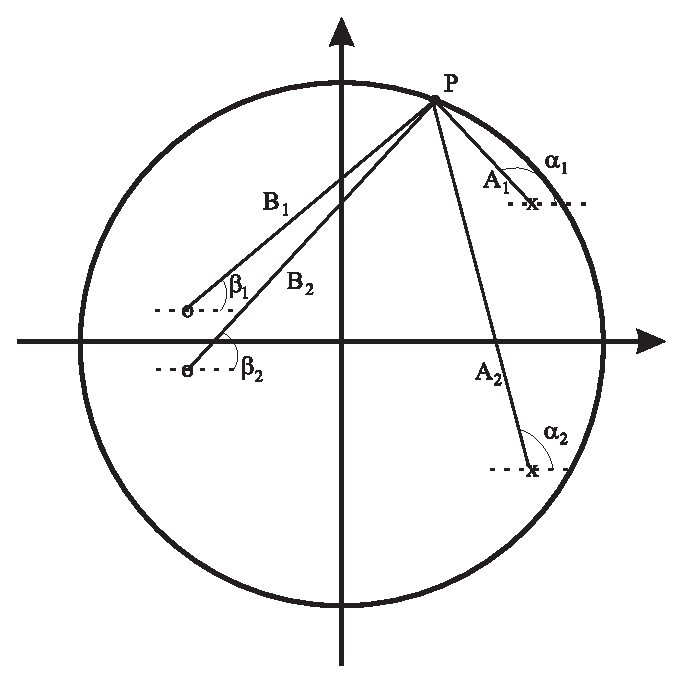
\includegraphics{psSpek/UebertragPolNullstellen}
\caption{\label{pic:SpecPolNullstellen}Skizze zur
Veranschaulichung des Einflusses von Polen und Nullstellen auf die
Übertragungsfunktion $H \jom$.}
\end{center}
\end{figure}

Um den Betrag des Frequenzganges an der Stelle $P$ zu berechnen,
müssen die Abstände der Pole und Nullstellen zu diesem Punkt $A_1,
A_2,B_1,B_2$ bekannt sein. Er ergibt sich
\begin{equation}\label{eq:spec:EInfacheBetragsrechnung}
    \left|H \jom\right|\Big|_{e^{j\Omega} = P} = |b_0| \frac{B_1 B_2}{A_1
    A_2}.
\end{equation}
Zusätzlich hat der Koeffizient $b_0$ einen Einfluss, der aber aus
dem Pol-Nullstellenplan nicht ersichtlich ist.

Die Phase an diesem Punkt kann durch
\begin{equation}\label{eq:spec:EenfachePhasenrechnung}
    \arg\left\{H \jom \right\}\Big|_{e^{j\Omega} = P} = -\arg\{b_0\}  + \beta_1 + \beta_2
    - \alpha_1 - \alpha_2
\end{equation}
berechnet werden. Da $b_0$ für reellwertige Systeme ebenfalls
reell ist, kann der Term $\arg\{b_0\}$ auch weggelassen werden, bzw.~führt bei negativem
$b_0$ zu einer Phasendrehung von $\pi$.

Für allgemeine Systeme mit einem Zählergrad $M$ und einem
Nennergrad $N$ ergibt sich \cite{KK98}.
\begin{equation}\label{eq:SpektrumBetragAllg}
    \left|H \jom\right| = |b_0| \frac{\displaystyle \prod_{i = 0}^{M-1} \sqrt{1-2|n_i|\cos(\Omega-\arg\{n_i\})+|n_i|^2}}
    {\displaystyle \prod_{i = 0}^{N-1}\sqrt{1-2|p_i|\cos(\Omega-\arg\{p_i\})+|p_i|^2}}
\end{equation}
bzw. für die Phase
\begin{eqnarray}\label{eq:SpektrumPhaseAllg}
    \arg\left\{H \jom\right\} &=& (M-N)\Omega - \arg\{b_0\} \\\nonumber
    && - \sum_{i = 0}^{M-1}\arctan\left\{\frac{\sin \Omega-|n_i|\sin(\arg\{n_i\})}{\cos \Omega-|n_i|\cos(\arg\{n_i\})}
    \right\}\\\nonumber
    && +\sum_{i = 0}^{N-1}\arctan\left\{\frac{\sin \Omega-|p_i|\sin(\arg\{p_i\})}{\cos \Omega-|p_i|\cos(\arg\{p_i\})} \right\}
\end{eqnarray}

\tbdb{Hier fehlt ein Beispiel, dass in Matlab erklärt wird}

\tbd{Phase muss noch deutlich besser erklärt werden, außerdem scheint die Phasenformel falsch zu sein}

Eine Interpretation führt zu den Schlüssen:
\begin{itemize}
    \item Je näher ein Pol am Einheitkreis liegt umso größer ist
    sein Einfluss auf die Übertragungsfunktion
    \item Eine Nullstelle auf dem Einheitskreis führt zu einem
    Phasensprung um $\pi$.
    \item Systeme, bei denen alle Nullstellen im inneren des 
    Einheitskreises liegen, heißen minimalphasig.
    \item Pole oder Nullstellen im Ursprung verändern nur die Phase, aber nicht den
    Betrag der Übertragungsfunktion.
    \item Nullstellen die am Einheitskreis gespiegelt werden $r_{out} = 1/r_{in}$,
    führen nur zu einer Veränderung der Grundverstärkung des Betrages der
    Übertragungsfunktion aber nicht zu einer Veränderung der Form. Gleichzeitig
    wird aber die Phase so verändert, dass sie um über $180^{\circ}$ dreht und das
    resultierende System nicht mehr minimalphasig ist.
    \item Systeme bei denen die Nullstellen an den Positionen der am Einheitskreis
    gespiegelten Pole liegen
    \begin{equation}\label{eq:AllpassGrundlagenFormel}
    n_{i_0} = \frac{1}{p_{i_{\infty}}}
    \end{equation}
    heißen Allpasssysteme, da der Betrag
    für alle Frequenzen konstant bleibt. Nur die Phase wird
    verändert und dreht um $N \pi$, wobei $N$ die Ordnung
    des Systems angibt.
\end{itemize}

\section{Diskrete Fourier-Transformation\label{sec:DFT}}
Zur Frequenzanalyse ist bisher nur die DTFT bekannt. Aber diese
Transformation kann nicht auf einem Computer umgesetzt werden, da
das resultierende Spektrum nicht diskret ist. Außerdem benötigt
man unendlich viele Eingangswerte um das Spektrum zu berechnen.
Deshalb wird in einem ersten Schritt die Anzahl der genutzten
Abtastwerte auf $N$ beschränkt. Man könnte dies auch so
interpretieren, dass die unendliche Folge des Signals mit einer
Rechteckfolge der Höhe eins und der Länge N multipliziert wird. Da
außerhalb des Eins-Bereichs alle Multiplikationen zu Null werden,
können auch die Summengrenzen verändert werden.

Diese Rechteckfolge werden wir im weiteren mit Fenster oder {\em
Window} bezeichnen, da es aus der Folge nur einen Ausschnitt
zeigt, in Anlehnung an ein Glasfenster , das uns nur einen
Ausschnitt der Wirklichkeit zeigt (siehe Abbildung
\ref{pic:DFT_FensterMult}). Die Länge $N$ nennen wir Blockgröße,
da nur noch ein Block an Daten verarbeitet wird.

\begin{figure}[H]
\begin{center}
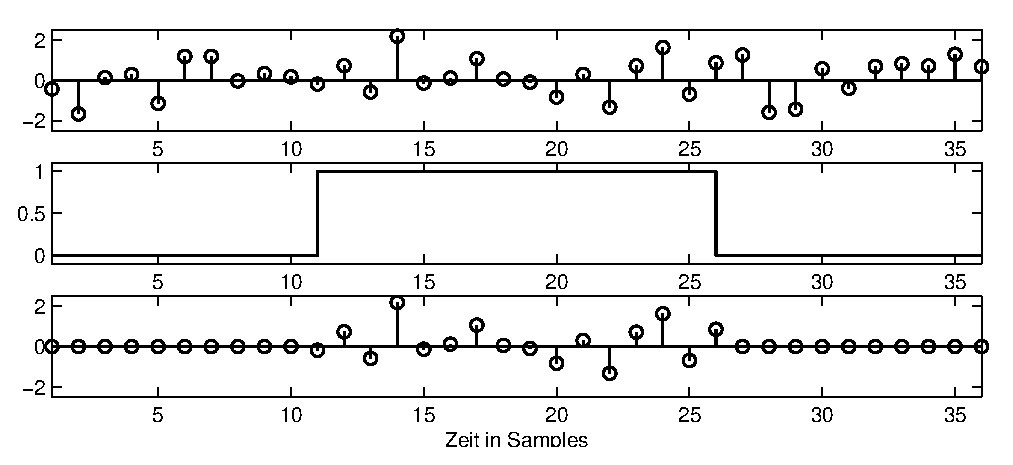
\includegraphics{psSpek/DFT_FensterMultiplikation}
\caption{\label{pic:DFT_FensterMult}Veranschaulichung der Wirkung
einer Rechteck-Fensterfunktion der Länge $N = 16$.}
\end{center}
\end{figure}

Das resultierende Spektrum ist aber immer noch kontinuierlich.
Durch die periodische Wiederholung des Spektrums ist es aber
ausreichend nur den Bereich von $0 \leq \omega\leq 2\pi $ genauer
zu betrachten. Um jetzt eine diskretes Spektrum zu erhalten,
unterteilen wir das Spektrum in $N$ gleichförmige
Abschnitte\footnote{Man kann auch eine andere Anzahl verwenden,
aber $N$ führt zu besonders effizienten Lösungen.}.

Die DTFT geht damit in
\begin{equation}\label{eq:DFTHin:Def}
    X(n) = X\left(e^{j 2 \pi n / N}\right) = \sum_{k = 0}^{N-1}x(k) e^{-j 2 \pi n k /N}
\end{equation}
über.

Umgekehrt ist es natürlich auch möglich, aus den $N$
Spektralwerten auch auf die Folge zurück zuschließen. Die
Rücktransformation enthält zusätzlich noch einen Normierungsterm
$N$ und unterscheidet sich sonst nur in dem Vorzeichen der
e-Funktion.
\begin{equation}\label{eq:DFTRueck:Def}
    x(k) = \frac{1}{N} \sum_{n = 0}^{N-1}X(n) e^{j 2 \pi n k /N}
\end{equation}

Das Transformationspärchen \ref{eq:DFTHin:Def} und
\ref{eq:DFTRueck:Def} werden als diskrete Fourier-Transformation
(DFT), bzw.\ inverse DFT (IDFT) bezeichnet.


\section{Eigenschaften}
\subsection{Zusammenhang DTFT und DFT}
Wir haben, um von der exakten Darstellung des Spektrums mittels
DTFT auf die computerlösbare DFT zu kommen, zwei Veränderungen
vorgenommen und natürlich spiegeln sich diese Veränderungen auch
im Ergebnis wieder. Wir müssen also versuchen, die Veränderungen
zu analysieren, um sicher zu sein, dass die DFT zumindest eine
Näherung der DTFT ist.

Zunächst ist es interessant die vorgenommene Diskretisierung im
Frequezbereich zu untersuchen. Im Grunde genommen haben wir das
Spektrum abgetastet. Die Konsequenz der Abtastung kennen wir
bereits aus der normalen Abtastung im Zeitbereich. Es kommt zu
einer periodischen Wiederholung des Spektrums. Die Abtastung im
Frequenzbereich führt zu einer periodischen Wiederholung im
Zeitbereich. Wenn man also ein Signal analysiert und zurück
transformiert ergibt sich eine periodische Wiederholung. Auch hier
gibt es eine andere Interpretationsmöglichkeit. Bei der
Analyse von periodischen Signalen mittels Fourier-Reihen ergeben
sich diskrete Spektren. Ein diskretes Spektrum führt im
Umkehrschluss also zu einer periodischen Zeitfunktion, wobei bei
der DFT die Periode genau $N$ ist (siehe Abbildung
\ref{pic:DFT_SignalPeriode}).

\begin{figure}[H]
\begin{center}
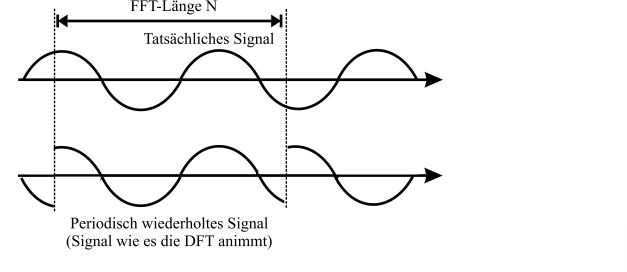
\includegraphics{psSpek/DFT_SignalPeriodizitaet}
\caption{\label{pic:DFT_SignalPeriode}Veranschaulichung der
erzwungenen Signal-Periodizität durch die DFT.}
\end{center}
\end{figure}

Der Einfluss der Fenster-Funktion lässt sich zunächst nur durch
die DTFT beschreiben. Es ist bekannt, dass eine Faltung im
Zeitbereich zu einer Multiplikation im Bildbereich
(Frequenzbereich) führt. Das Umgekehrte gilt aber auch. Eine
Multiplikation im Zeitbereich, und die Nutzung des Fensters ist
eine Multiplikation, führt im Frequenzbereich zu einer Faltung der
Spektren, wobei die Faltung hier kontinuierlich als Integral zu
definieren ist, da wir ja ein kontinuierliches periodisches
Spektrum haben.
\begin{equation} \label{eq:SpektrumBegrenzterFolgen}
    H \jom \Big|_{0 \leq n \leq N} = \int_{\theta = -\pi}^{\pi} H
    (e^{j\theta}) H^{W}(e^{j(\Omega - \theta)})d\theta
\end{equation}
wobei $H^{W}$ die Übertragungsfunktion der Fensterfunktion ist.

Für das Rechteckfenster ergibt sich das Spektrum, indem
wir zunächst die z-Transformation der Fensterfolge $w(k)$ ansetzen
Es gilt:
\[
    H^{W}(z) = \sum_{k = -\infty}^{\infty} w(k) z^{-k} = \sum_{k = 0}^{N-1} z^{-k}
\]
Durch einsetzen von $z = e^{j\Omega}$ ergibt sich das Spektrum
\[
    H^{W}(z)\Big|_{z = e^{j\Omega}} = \sum_{k = 0}^{N-1} e^{-j\Omega k}
\]
mit der Formel der endlichen geometrischen Reihe\footnote{
\[
    1+x + x^2 + \cdots + x^{N-1} = \frac{1-x^N}{1-x}
\]}
erhält man das Spektrum der Rechteckfunktion:
\begin{eqnarray}
    H^{W}\jom & = & \frac{1-e^{-j\Omega N}}{1- e^{-j\Omega}}\\
    & = & \frac{e^{-j\Omega N/2} \overbrace{(e^{j\Omega N/2}- e^{-j\Omega N/2})}^{2j\sin(\Omega N/2)}}
    {e^{-j \Omega/2}\underbrace{(e^{j \Omega/2}- e^{-j\Omega/2})}_{2j\sin(\Omega/2)}}\\
    & = & e^{-j(N-1)\Omega/2}\frac{\sin\left(N \Omega/2
\right)}{\sin\left(\Omega/2 \right)}
\end{eqnarray}
Der vordere Teil dieser Funktion entspricht einer linearen
Phasenverschiebung. Der zweite Teil mit den Sinustermen stellt
eine sogenannte Dirichlet-Funktion dar. Der Betrag dieser Funktion ist in
Abbildung \ref{pic:DirichletFkt} gezeigt.

\begin{figure}[H]
\begin{center}
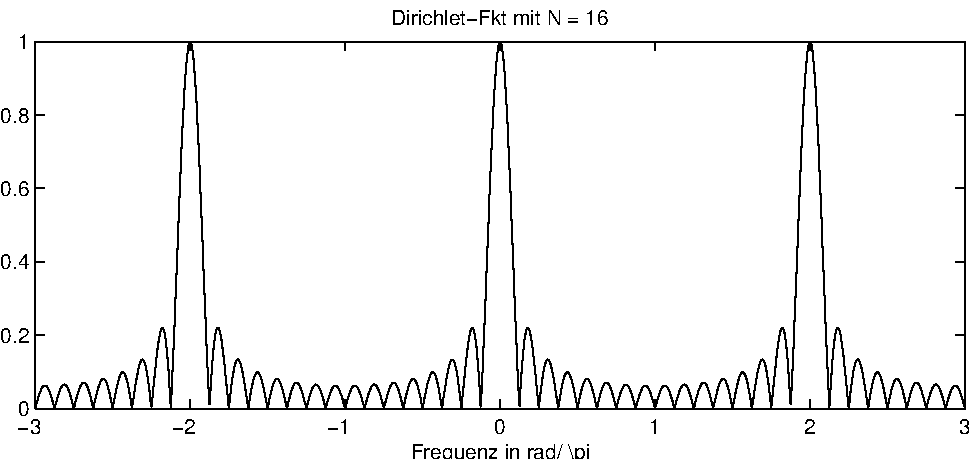
\includegraphics[width = 10cm]{psSpek/DirichletFkt}
\caption{\label{pic:DirichletFkt}Betrag von $H^{W}\jom$ für $N = 16$.}
\end{center}
\end{figure}

\begin{example}
DTFT und DFT bei einer Cosinus-Schwingung\\
Um die Unterscheide zwischen DTFT und DFT bei der Spektrumsberechnung
eines Cosinus müssen wir zunächst das Spektrum einer abgetasteten Cosinus-Schwingung berechnen:
\begin{eqnarray}
H \jom & = & \sum_{-\infty}^{\infty} \cos \left(k \Omega_0  \right) e^{-j\Omega k}\\
       & = & \sum_{-\infty}^{\infty} \frac{1}{2}\left( e^{j k \Omega_0} + e^{-j k \Omega_0}\right) e^{-j\Omega k}\\
       & = & \sum_{-\infty}^{\infty} \frac{1}{2} \left( e^{j k (\Omega_0-\Omega)} + e^{-j k (\Omega_0 + \Omega)}\right)\\
       & = & \sum_{-\infty}^{\infty} \frac{1}{2} e^{-j k (\Omega-\Omega_0)}
       + \sum_{-\infty}^{\infty} \frac{1}{2} e^{-j k (\Omega + \Omega_0)}\\
       & = & \frac{1}{2} \Dirac{\Omega - \Omega_0}
       + \frac{1}{2} \Dirac{\Omega + \Omega_0}
\end{eqnarray}
mit $\Omega = 2\pi f / f_s$.
Das heißt, das Spektrum des abgetasteten Cosinus hat nur zwei definierte
Frequenzwerte, an den Frequenzen $\Omega = \pm \Omega_0$.
\end{example}

Um den Einfluss der Annäherung durch die DFT zu veranschaulichen, begrenzen wir den
betrachteten Signalausschnitt auf $N$ Datenwerte. Dies führt wie in Gleichung
\ref{eq:SpektrumBegrenzterFolgen}
gezeigt zu einer Faltung mit dem Spektrum des Rechtecks. Durch die Siebeigenschaft
der $\delta$-Funktion ergibt sich
\begin{eqnarray}
    H \jom & = & \left(\frac{1}{2} \delta \left(\Omega - \Omega_0 \right)
       + \frac{1}{2} \delta \left(\Omega + \Omega_0 \right) \right) \ast H^{W} \jom \\
           & = & \frac{1}{2} H^{W} \left(e^{j(\Omega -\Omega_0 )}\right) +
                 \frac{1}{2} H^{W} \left(e^{j(\Omega + \Omega_0 )}\right).
\end{eqnarray}
Das Spektrum des Rechtecks wird also, um $\pm \Omega_0$ verschoben.
Abbildung \ref{pic:VerschobesRechteckSpektrum} zeigt
das resultierende Spektrum für $N = 16$ bei einer Grundfrequenz von 155Hz und einer Abtastrate von
$f_s = 1$kHz.

\begin{figure}[H]
\begin{center}
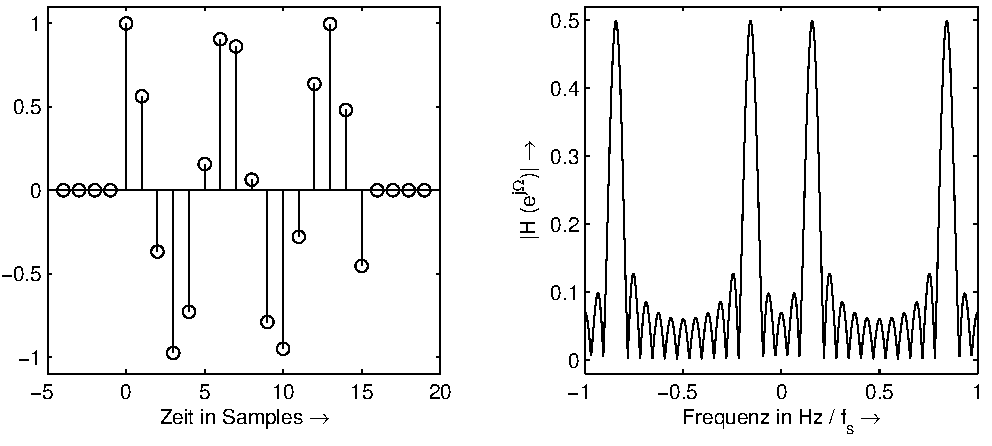
\includegraphics[width = 10cm]{psSpek/DFT_Cosinus}
\caption{\label{pic:VerschobesRechteckSpektrum}Spektrum (Rechts) einer abgetasteten Cosinus-Fkt., die auf
$N = 16$ Werte begrenzt wird (Links) ($f_s = 1 $kHz und $f_0 = 155$Hz).}
\end{center}
\end{figure}

Um nun das DFT-Spektrum zu berechnen ist zusätzlich die Abtastung im Frequenzbereich notwendig.
Dies hat implizit zur Folge, dass die Cosinusfolge periodisch wiederholt wird. Das
abgetastete Spektrum ist auf der linken Seite in
Abbildung \ref{pic:VerschobesRechteckSpektrumAbgetastet} zu sehen und die resultierende Folge
auf der rechten Seite.

\begin{figure}[H]
\begin{center}
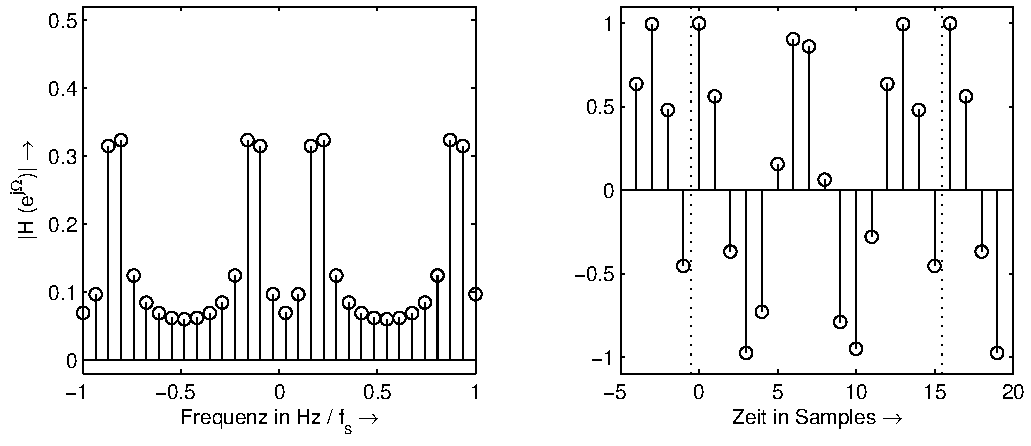
\includegraphics[width = 10cm]{psSpek/DFT_CosinusSpektrum}
\caption{\label{pic:VerschobesRechteckSpektrumAbgetastet}Abgetastetes Spektrum (Links)
und die daraus resultierende periodisch fortgesetzte Cosinus-Fkt mit Sprungstellen (rechts).}
\end{center}
\end{figure}

Das resultierende Spektrum hat nicht das erwartete Maximum bei $f_0$, da $155Hz$ nicht
im Abtastraster einer 16 Punkte FFT bei einer Abtastrate von 1kHz liegt. Statt dessen ist
die Leistung des Cosinus über viele Abtastpunkte spektral verteilt. Dieser Effekt wird auch als
{\em Leakage} bezeichnet.

\tbd{Beispiele mit anderen Frequenzen, um zu zeigen, dass Dirichlet-Funktion abgetastet wird.}


\subsection{Symmetrien der DFT}
Eine der wichtigsten Symmetrien für die diskrete sowie für die
zeitdiskrete Fourier-Transformation (DFT und DTFT) ergibt sich für
reelle Signale. Aus den Eigenschaften der z-Transformation ist
deutlich, dass sich nur dann reelle Koeffizienten bei Signalen und
Systemen ergeben, wenn die Pole und Nullstellen konjugiert komplex
auftreten. Daraus ergibt sich, dass die Spektren reeller Signale
konjugiert komplex sind. Es ergibt sich also eine Symmetrie der
Spektren an der Null Hertz (Gleichstrom) Linie. Der Realteil ist
dabei achsensymmetrisch (gerade) und der Imaginärteil punktsymmetrisch (ungerade).
Diese Symmetrien ergeben sich auch, wenn Betrag und Phase
betrachtet werden. Der Betrag reeller Funktionen ist immer
achsensymmetrisch und die Phase punktsymmetrisch (siehe Abbildung \ref{pic:SymmetrienDFT})
\begin{figure}[H]
\begin{center}
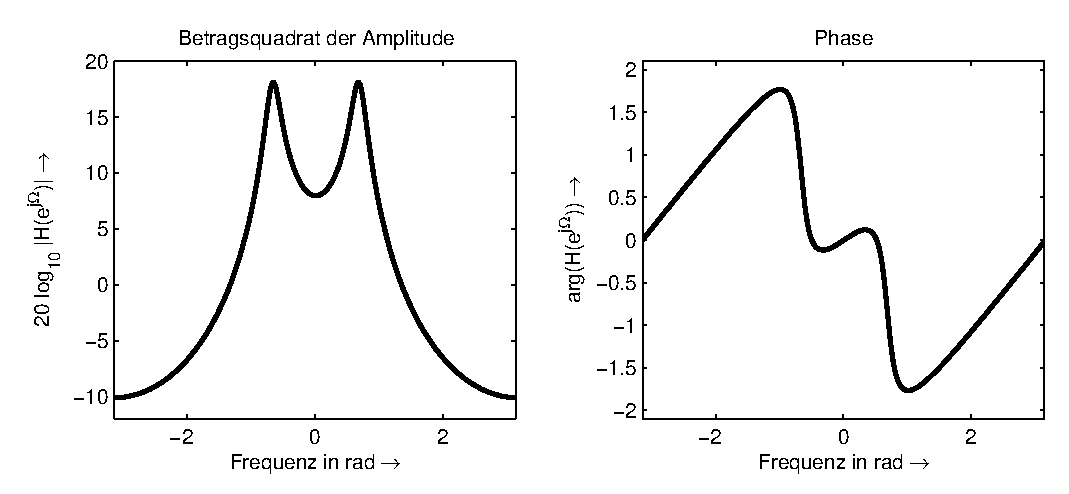
\includegraphics[width = 10cm]{psSpek/SymmetriePlot}
\caption{\label{pic:SymmetrienDFT}Beispiel eines Frequenz- und Phasenverlaufs eines reellwertigen Systems.}
\end{center}
\end{figure}

Die Symmetrien lassen sich bei der Berechnung der DFT und IDFT
ausnutzen, da immer nur das halbe Spektrum berechnet werden muss,
während die andere Hälfte durch Spiegelung erzeugt werden kann.
Häufig kommt es vor, dass man im Spektralbereich etwas berechnet
und an der dazugehörigen Zeitfolge interessiert ist (zum Beispiel
beim Filterentwurf). Es reicht aus, für eine $N$-Punkte DFT,
$N/2+1$ Spektralwerte zu kennen. Man benötigt einen Wert mehr, da
die DFT für die höchste Frequenz bei $f_s/2$ nur einen
reellwertigen Koeffizienten besitzt. Die Kopievorschrift in Matlab
sieht dann wie folgt aus, wobei wir annehmen, die $N/2+1$ Werte
sind in \verb/H_halb/ gespeichert
\begin{verbatim}
H_voll = [H_halb conj(H_halb(end-1:-1:2))];
\end{verbatim}
Die Gegenprobe, ob alle Symmetrien richtig aufgebaut wurden, ist
das Überprüfen, ob nach der Rücktransformation eine rein
reellwertige Folge entsteht, wobei bei Matlab durch Rundungsfehler
immer die resultierende Variable komplex ist. Es ist deshalb immer
notwendig, den Betrag des Imaginäranteils zu überprüfen. Dieser
sollte sehr kleine Werte um $10^{-7}$ nicht überschreiten.

Wie lässt sich die Symmetriebedingung mathematisch zeigen?

Ausgehend von
\[
    X(n) = \sum_{k = 0}^{N-1} x(k) e^{-jkn2\pi/N}
\]
ergibt sich für die an der y-Achse gespiegelte Folge durch Variablensubstitution
\[
    X(-n) = \sum_{k = 0}^{N-1} x(k) e^{jkn2\pi/N}
\]
Konjugiert man dieses Signal ergibt sich
\begin{eqnarray}
    X^{\ast}(-n)  &  =  & \sum_{k = 0}^{N-1} \underbrace{x^{\ast}(k)}_{=x(k)\:\mbox{, da reell}}
    \underbrace{e^{-jkn2\pi/N}}_{\mbox{Beachte -}}\\
                  &  =  & X(n)
\end{eqnarray}

\subsubsection{Spektren reeller gerader Folgen}
Die Symmetriebedingung reeller gerader Folgen kann aus den vorherigen
Überlegungen geschlossen werden. Da gerade Funktionen achsensymmetrisch
sind, der Imaginärteil aber punktsymmetrisch, können wir schließen, dass
reelle, gerade Funktionen ein reelles, gerades Spektrum haben.

%\subsubsection{Weitere Symmetrien}

%\tbd{gerade / ungerade}

%Allgemein lässt sich für die einzelnen Teile eines komplexen Signals, die folgenden
%korrespondierenden Spektren finden.

%\tbd{Bild mit Transkreuz, siehe Girod}

\subsection{Rechenregeln}
\subsubsection{Linearität}
Die DFT ist eine lineare Transformation. Es gilt also das
Superpositionsprinzip:
\begin{equation}\label{eq:DFT:Linearitaet}
  a_1 x_1(k) + a_2 x_2(k) \HinTrans a_1 X_1(n) + a_2 X_2(n)
\end{equation}

\subsubsection{Faltung \label{sec:DFT:Faltung}}
Bisher haben wir bereits die Faltung bei der z-Transformation kennen gelernt und
den Übergang der Faltung in die Multiplikation in der z-Ebene. Dieser Zusammenhang
gilt auch für die DTFT, aber nicht so direkt für die DFT. Um das zu veranschaulichen,
kann ein einfaches Beispiel dienen. Gehen wir davon aus, dass wir eine Folge mit $N = 8$
Werten mit Hilfe der DFT in den Bildbereich transformieren. Wir erhalten 8 Frequenzpunkte.
Des Weiteren transformieren wir eine zweite Folge mit 8 Datenwerten. Wir erhalten
erneut 8 Spektralwerte. Multiplizieren wir diese beiden Spektren und führen eine
Rücktransformation durch, so besteht das Ergebnis auch aus 8 Werten im Zeitbereich.
Aus der Faltungsalgebra wissen wir aber, dass das Faltungsprodukt aus $L+M-1$
Elementen bestehen muss, in diesem Beispiel also 15 Datenwerte. Daraus folgt, dass die
Faltung nicht der Multiplikation mit den DFT-Spektralwerten entspricht.

Die Ursache hierfür ist in der implizierten Periodizität der DFT zu finden. Das DFT Spektrum
ist gerade nicht das Signal im betrachteten Zeitfenster, sondern ein Signal das periodisch
fortgesetzt ist. Die Multiplikation im Frequenzbereich führt deshalb auf eine Faltung dieser
periodisch fortgesetzten Sequenzen. Dies führt dazu, dass auch das Faltungsprodukt periodisch ist.
Man spricht deshalb von der zyklischen Faltung. Das Ergebnis kann sich vollständig von dem
gewünschten Ergebnis unterscheiden. Dies wird in Abbildung \ref{pic:BspZyklischeFaltung} demonstriert.
Die beiden Folgen (a,b) ergeben bei der Faltung im Zeitbereich die Folge c. Die Lösung mit Hilfe der
DFT führt auf die Folge d.

\begin{figure}[H]
\begin{center}
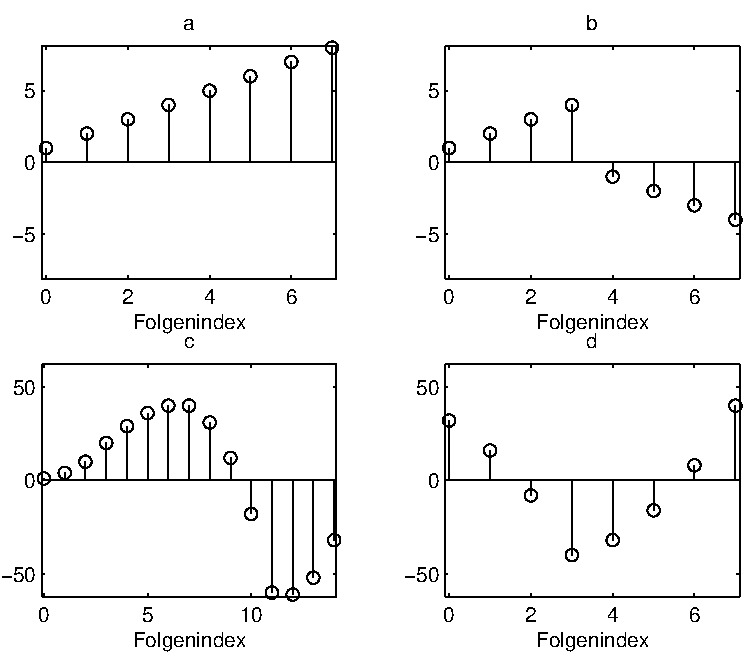
\includegraphics[width = 10cm]{psSpek/BspZyklischeFaltung}
\caption{\label{pic:BspZyklischeFaltung}Beispiel für zyklische Faltung. Die beiden Folgen (Bild a,b)
ergeben bei konventioneller Faltung Bild c. Bild d zeigt das Resultat für die direkte Faltung im
Frequenzbereich mit Hilfe der DFT.}
\end{center}
\end{figure}

Um die zyklischen Faltungsprodukte zu verhindern ist es notwendig Nullen an die
zu transformierenden Folgen anzuhängen ({\em Zero-Padding}) und eine entsprechend größere
Transformationslänge zu wählen. Dies führt dazu, dass die implizite Periodizität
die Nullen einschließt. Die Nullen verändern das Spektrum nicht, sondern nur die
Frequenzauflösung\footnote{Es enstehen keine genaueren Spektralwerte gegenüber der kurzen Folge.
Die Werte bei der höheren Frequenzauflösung könnten auch aus einer Interpolation
des Spektrums mit geringrer Auflösung gewonnen werden.}. Die Rücktransformation führt zu der
gewünschten Faltungsfolge, wobei durch die vorher eingebrachten Nullen
keine zyklischen Faltungsprodukte das Ergebnis
verfälschen. Bei dem obigen Beispiel würde sich das Ergebnis in Abbildung \ref{pic:BspZyklischeFaltung}c
ergeben, wenn an die Folgen a und b jeweils 8 Nullen angehängt werden und die DFT Länge auf 16
erhöht wird.

\tbd{Einfacheres Beispiel mit Rechteck und Dreiecksfunktionen, bei denen die
Wiederholungen eingezeichnet sind.}


\subsubsection{Theorem von Parseval}
Das Theorem von Parseval sagt aus, dass man die Energie eines Signals im Zeit, oder
im Frequenzbereich berechnen kann, bzw. dass die Leistung eines Signals im Zeit- und Frequenzbereich gleich ist.
Es gilt also für die DTFT:
\begin{equation}\label{eq:ParsevalDTFT}
    \sum_{k = -\infty}^{\infty} x^2(k) = \frac{1}{2\pi} \int_{-\pi}^{\pi} \left|X \jom \right|^2 d\Omega
\end{equation}
bzw. für die DFT
\begin{equation}\label{eq:ParsevalDFT}
    \sum_{k = 0}^{N-1} x^2(k) = \frac{1}{N}\sum_{n = 0}^{N-1} |X(n)|^2
\end{equation}



\subsection{Effiziente Implementierung}
Die DFT lässt sich durch Ausnutzung unterschiedlicher Symmetrien
sehr effizient berechnen. Um dies zu verdeutlichen, soll das sog.
{\em Decimation in Time}-Verfahren zur drastischen Reduktion der
benötigten Rechenleistung, genauer gezeigt werden. Andere
Verfahren können in der sehr umfangreichen Literatur zur
Entwicklung der sog. Fast Fourier Transform (FFT) gefunden werden
\cite{Coo90, KK98,OS99}

Um eine effiziente Realisierung zu finden, legen wir die Länge der
FFT so fest, dass sie eine 2er Potenz darstellt. Besonders häufig in der
Audio und Sprachsignalverarbeitung
genutzte FFT-Längen sind 256 , 512, 1024 und 2048.
Durch diese Forderung ist es möglich, die Folge in zwei Teilfolgen zu zerlegen, wobei
wir immer abwechselnd die Elemente der Folge, den jeweiligen neuen Teilfolgen zuordnen.
Es ergeben sich die Folgen $x(2k)$ und $x(2k+1)$ (siehe Abbildung \ref{pic:DecimationInTime}).

\begin{figure}[H]
\begin{center}
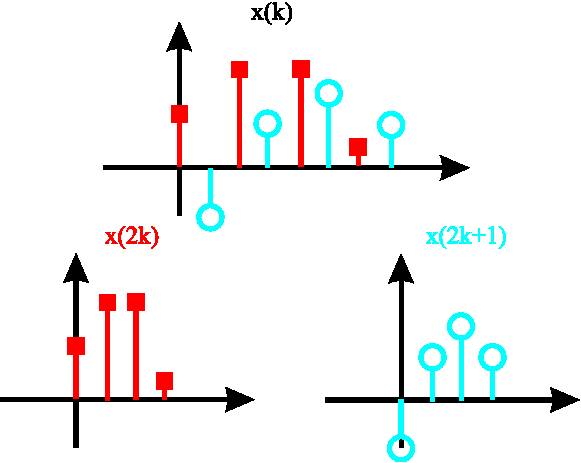
\includegraphics[width = 8cm]{psSpek/DecimationInTime}
\caption{\label{pic:DecimationInTime}Aufteilung einer Sequenz in zwei Teilsequenzen zur
Erklärung der FFT (Decimation in Time)}
\end{center}
\end{figure}

Die Konsequenzen für die DFT lassen sich nun wie folgt berechnen:
\begin{eqnarray} \nonumber
\sum_{k = 0}^{N-1} x(k) e^{-j 2 \pi n k /N} & = &
\sum_{k = 0}^{\frac{N}{2}-1} \underbrace{x(2k)}_{u(k)} e^{-j 2 \pi n 2k /N} +
\sum_{k = 0}^{\frac{N}{2}-1} \underbrace{x(2k+1)}_{v(k)} e^{-j 2 \pi n (2k+1) /N} \\\nonumber
& = & \underbrace{\sum_{k = 0}^{\frac{N}{2}-1}u(k) e^{-j 2 \pi n k /\frac{N}{2}}}_{U(n) \qquad \mbox {N/2 DFT}} +
e^{-j2\pi n /N} \underbrace{\sum_{k = 0}^{\frac{N}{2}-1}
v(k) e^{-j 2 \pi n k /\frac{N}{2}}}_{V(n) \qquad \mbox {N/2 DFT}}\\
X(n) & = & U(n) + e^{-j2\pi n /N} V(n)
\end{eqnarray}
Die N-Punkte DFT lässt sich also in zwei N/2-Punkte DFT zerlegen. Hierbei tritt jetzt das Problem auf,
dass die Folgen $U(n)$ und $V(n)$ nur bis $N/2$ definiert sind, da ja auch nur eine N/2 DFT durchgeführt wurde.
Die Lösung für dieses Problem ist durch die Periodizität der DFT aber sehr einfach zu umgehen, da sich das
Spektrum immer wiederholt.

Aber warum stellt es einen Vorteil dar, wenn man die DFT so zerlegen kann? Dazu müssen wir überlegen,
wie viele Multiplikationen notwendig sind um eine diskrete Frequenz zu berechnen. Es sind
$N$ komplexe Multiplikatinen nötig. Dieser Schritt muss für alle diskreten Frequenzen durchgeführt werden.
Die Berechnung des vollständigen Spektrums benötigt also $N^2$ Multiplikationen. Teilen wir die
Aufgabe in zwei Teilspektren benötigt man $2\left(\frac{N}{2}\right)^2$ + $N$ Multiplikationen für
den Drehfaktor vor $V(n)$. Im Vergleich ergeben sich \zB für $N = 8$ einmal 64 Multiplikationen
und für die aufgeteilten Spektren 40 Multiplikationen. Der Schritt der Aufteilung kann nun solange
wiederholt werden, bis die Folge nicht weiter aufgeteilt werden kann ($N = 2$). Zusätzlich
können einige Multiplikationen vernachlässigt werden, da $e^{j0} = 1$ ist. Eine
Reduktion auf $\frac{N}{2}\left( ld \frac{N}{2} \right)$ ist so möglich\footnote{ld bezeichnet den
Logarithmus zur Basis 2 (logarithmus dualis). }. Somit ergibt sich eine in der Rechenleistung
stark reduzierte DFT, die als {\em Fast Fourier Transform} (FFT) bekannt ist\footnote{In Matlab wird
die DFT durch den Befehl FFT aufgerufen.}.

\section{Spezielle Signale und ihre Spektren}

\subsubsection{Spektrum für $\delta(k)$}
Berechnet man die DTFT für den $\delta$-Impuls ergibt sich
\begin{equation}\label{eq:SpektrumDeltaImpuls}
    X \jom = \sum_{k = -\infty}^{\infty} \delta(k)e^{-jk \Omega} =e^{-j0 \Omega} = 1,
\end{equation}
da der $\delta$-Impuls ausschließlich an der Stelle $k = 0$ definiert ist.
Das Betrag des Spektrums ist also eins für alle Frequenzen und die Phase ist null
für alle Frequenzen.

\subsubsection{Spektrum für $\delta(k-k_0)$}
Der um $k_0$ verschobene $\delta$-Impuls führt zu einem etwas anderem Spektrum
\begin{equation}\label{eq:SpektrumDeltaImpuls}
    X \jom = \sum_{k = -\infty}^{\infty} \delta(k-k_0)e^{-jk \Omega} =e^{-jk_0 \Omega}.
\end{equation}
Das Spektrum ist im Betrag ebenfalls Eins für alle Frequenzen, aber die Phase des Signals
wird linear abhängig von der Frequenz verändert, wenn ein $\delta(k)$ ein System darstellt

%\subsubsection{Spektrum für $\gamma(k)$}

%\tbd{Nachschlagen}

\section{Weitere Fensterfunktionen und deren Eigenschaften}
Wir haben gesehen, dass die DFT für eine zeitlich beschränkte
Funktion auch als Multiplikation mit einer Fensterfunktion
interpretiert werden kann. Dieses Fenster hatte einen deutlichen
Einfluss auf das dargestellte Spektrum. Zur Beschreibung der
Eigenschaften des Fensters im Frequenzbereich wird häufig die
spektrale Auflösung des Maximums zu den 3dB Punkten verwendet.
Weiterhin ist eine interessante Größe, welche Höhe die nächsten
Maxima haben (Betrag). Für das Rechteckfenster sind diese beiden
Größen durch $2pi/N$ und $\approx 13$dB gegeben. Etwas anders sieht
dies bei anderen Fensterfunktionen aus (siehe Abbildungen
\ref{pic:HannWindow} - \ref{pic:KaiserFenster2}).
\begin{figure}[H]
\begin{center}
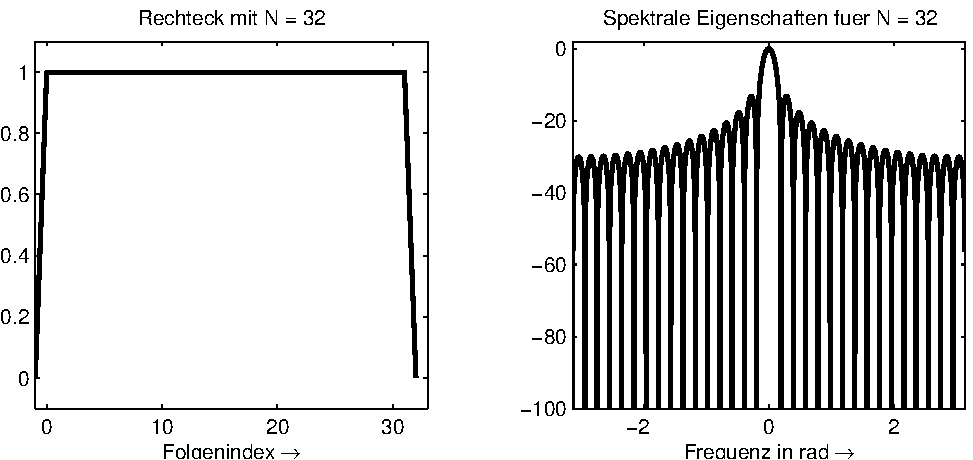
\includegraphics[width = 11cm]{psSpek/RechteckWindow}
\caption{\label{pic:RectWindow}Zeitliche und spektrale Eigenschaft
des Rechteckfensters}
\end{center}
\end{figure}

Als Ursache für das verschmieren im Frequenzbereich wurde die
Faltung mit der Fensterfunktion genannt. Die Ursache im
Zeitbereich hierfür war das abrupte Abschneiden, dass durch die
angenommene zirkulare WIederholung zu einem nicht-repräsentativen
Ausschnitt führte. Deshalb ist eine Design-Idee für andere Fenster
eine möglichst weiche Ausblendung zu den Rändern zu ermöglichen.
Fenster die diese Eigenschaft besitzen können zum Beispiel durch
Cosinusfunktionen realisiert werden.

Eine generalisierte Version ergibt sich dabei zu
\begin{equation}\label{eq:WindowFunction:General}
   w(k) = \alpha - \beta \cos(2\pi k /N) + \gamma \cos(4\pi k /N) \quad \Mit \quad 0\leq k
   < N
\end{equation}

Durch Veränderung der drei Parameter $\alpha, \beta, \gamma$
können die bekanntesten Fenster-Funktionen angegeben
werden\footnote{Bei der Darstellung wurden die jeweiligen
Übertragungsfunktionen auf ihr Maximum normiert, so dass sich
immer ein Hauptmaxima mit 0dB ergibt.}.
\begin{itemize}
    \item {\bf von Hann- Fenster:\footnote{Oft auch fälicherweise als Hanning-Fenster
    bezeichnet}} Für das Hann-Fenster ist $\alpha = \beta = 0.5$
    und $\gamma = 0$. Daraus ergibt sich im Frequenzbereich ein
    etwas breiteres Hauptmaxima $4\pi/N$. Die Nebenmaxima sind dafür im
    Gegensatz zum Rechteck-Fenster sehr viel stärker bedämpft.
\begin{figure}[H]
\begin{center}
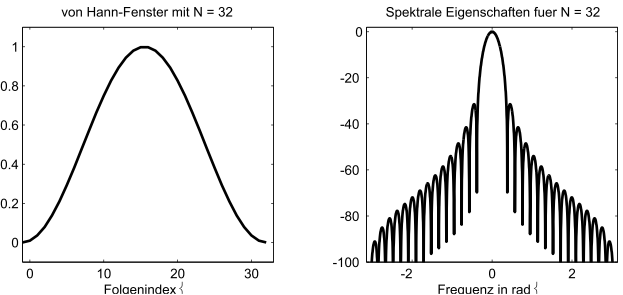
\includegraphics[width = 11cm]{psSpek/HannWindow}
\caption{\label{pic:HannWindow}Zeitliche und spektrale Eigenschaft
des von Hann-Fensters}
\end{center}
\end{figure}

    \item {\bf Hamming- Fenster:} Für das Hamming-Fenster ist $\alpha = 0.54$, $\beta = 0.46$
    und $\gamma = 0$. Das Design-Ziel des Hamming-Fenster ist das
    erste Nebenmaxima möglichst optimal zu unterdrücken. Dafür
    geht aber insgesamt eine schlechtere Dämpfung der
    anderen Nebenmaxima einher. Die Verbreiterung entspricht der
    des Hann-Fensters $4\pi/N$
\begin{figure}[H]
\begin{center}
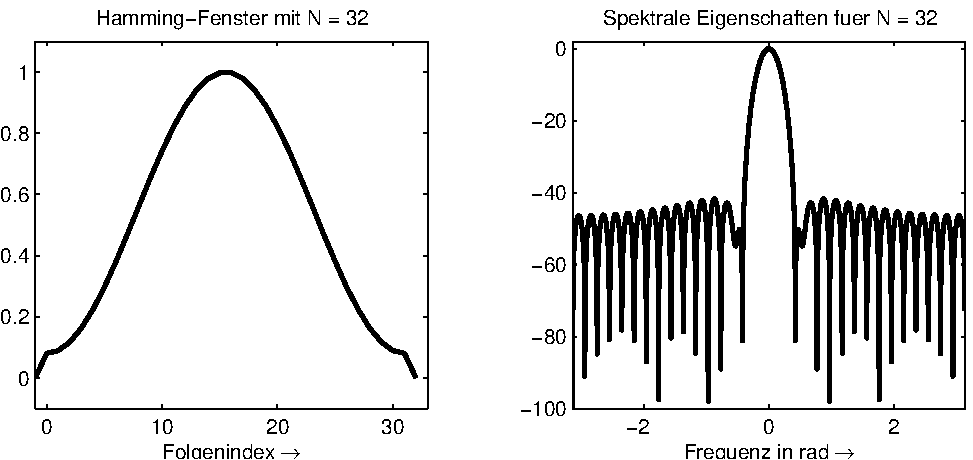
\includegraphics[width = 11cm]{psSpek/HammingWindow}
\caption{\label{pic:HammingWindow}Zeitliche und spektrale Eigenschaft
des Hamming-Fensters}
\end{center}
\end{figure}
    \item {\bf Blackman- Fenster:} Für das Blackman-Fenster ist $\alpha = 0.42$, $ \beta = 0.5$
    und $\gamma = 0.08$. Dieses Fenster hat eine deutlich breitere
    Hauptkeule $6\pi/N$, aber die Dämpfung der Nebenmaxima und der Abfall
    der weiteren Nebenmaxima ist sehr hoch.
\begin{figure}[H]
\begin{center}
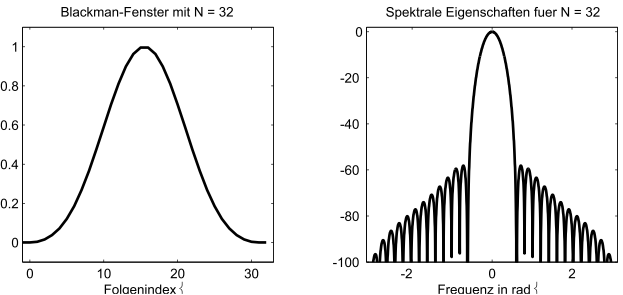
\includegraphics[width = 11cm]{psSpek/BlackmanWindow}
\caption{\label{pic:BlackmanWindow}Zeitliche und spektrale Eigenschaft
des Blackman-Fensters}
\end{center}
\end{figure}
    \item {\bf Dolph-Chebbyscheff Fenster:} Im Gegensatz zu den anderen Fenstern in das
    Dolph-Chebbycheff Fenster parametrisierbar. Bei einer vorgegebenen Fensterlänge $N$ kann die
    Absenkung der Nebenzipfel angegeben werden. Dieser Wert wird für alle Nebenzipfel
    gleichmäßig erreicht. Die Breite der Hauptkeule wird gleichzeitig optimal klein für eine
    gegebene Fensterlänge $N$.
    Siehe auch in Matlab \verb/chebwin/
\begin{figure}[H]
\begin{center}
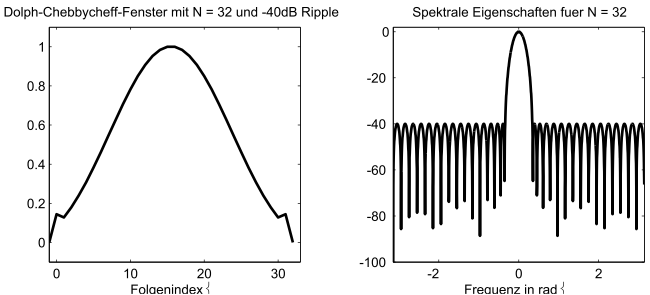
\includegraphics[width = 11cm]{psSpek/ChebWindow}
\caption{\label{pic:ChebWindow}Zeitliche und spektrale Eigenschaft
des Dolph-Chebbycheff-Fensters}
\end{center}
\end{figure}

    \item {\bf Kaiser Fenster:} Auch das Kaiser Fenster ist mit Hilfe des Parameters $\alpha$
    veränderlich. Es basiert auf der Form
\begin{equation}\label{eq:Kaiser-Fenster}
   w(k,\alpha) = \left\{\begin{array}{c}
     \frac{I_0\left(\alpha \sqrt{1-(k/N)^2}\right)}{I_0 (\alpha)}     \quad \Mit \quad 0\leq k
   < N\\
     0 \quad \quad \mbox{sonst} \\
   \end{array}
   \right.
\end{equation}
wobei $I_0$ die modifizierte Bessel-Funktion nullter Ordnung darstellt.

Abbildung \ref{pic:KaiserFenster} und \ref{pic:KaiserFenster2} zeigen für
unterschiedliche $\alpha$ den zeitlichen Verlauf und die dazugehörigen spektralen Eigenschaften.
\begin{figure}[H]
\begin{center}
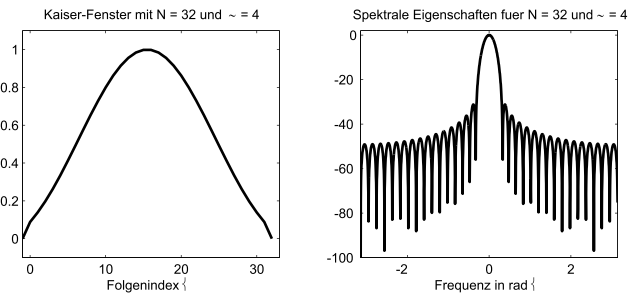
\includegraphics[width = 11cm]{psSpek/KaiserWindow}
\caption{\label{pic:KaiserFenster}Zeitliche und spektrale Eigenschaft
des Kaiser-Fensters mit $\alpha = 4$.}
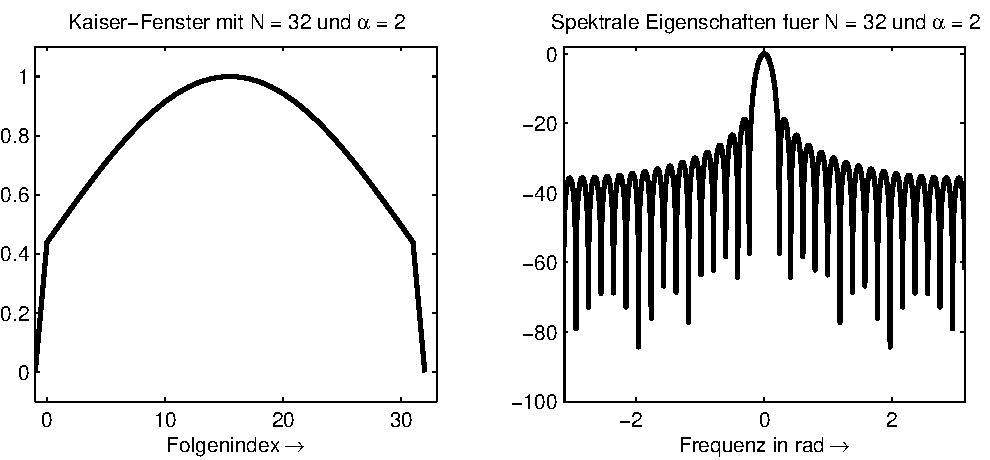
\includegraphics[width = 11cm]{psSpek/KaiserWindow2}
\caption{\label{pic:KaiserFenster2}Zeitliche und spektrale Eigenschaft
des Kaiser-Fensters mit $\alpha = 2$.}
\end{center}
\end{figure}
\end{itemize}

\tbd{Vergleichstabelle der Fensterfunktionen, Hinweise für Applikationen}

\compileif{bBook}
{
\section{Matlab und Spektren}
siehe Matlab Versuch drei.
\subsection{Fenster-Funktionen}
\subsection{FFT}
\subsection{Signalanalyse}
}
\section{Übungen}
\subsection{Wiederholung des Stoffes und einfache Rechenaufgaben}
\begin{enumerate}
    \item Bei einer Abtastrate von 44100 Hz und einer DFT Auflösung von $1024$ soll
    ein Sinus erzeugt werden, der keinerlei Leck-Effekt zur Folge hat. Welche Frequenzen sind
    mögliche Kandidaten.
    \item Wozu werden Fensterfunktionen benötigt?
    \item Nach welchem Prinzip kann die Rechenleistung der DFT reduziert werden?
    \item Welchen Einfluss haben Pole auf das Übertragungsverhalten und welchen Einfluss Nullstellen?
    \item Wodurch entsteht ein Allpass-System?
    \item Erklären Sie, die Folgen des Übergangs von der DTFT zur DFT!
    \item Um zu zeigen, dass nicht-lineare Systeme neue Frequenzen
    erzeugen, sollten Sie das System $y(k) = x^2(k)$ mit der
    Exponentialschwingung anregen und sich das Ergebnis anschauen
    \item Ein mit 200Hz abgetastetes reelles Signal wird mit einer 8 Punkte
    DFT spektral analysiert. Welche Frequenzbereiche sind in den 8
    Spektralwerten enthalten? Welche dieser Werte (Indize) haben den gleichen
    Betrag?
    \item {Zeichnen Sie qualitativ die Betragsübertragungsfunktion für die folgenden durch
    einen Pol-Nullstellenplan gegebenen Systeme:
   \begin{figure}[H]
    \begin{center}
    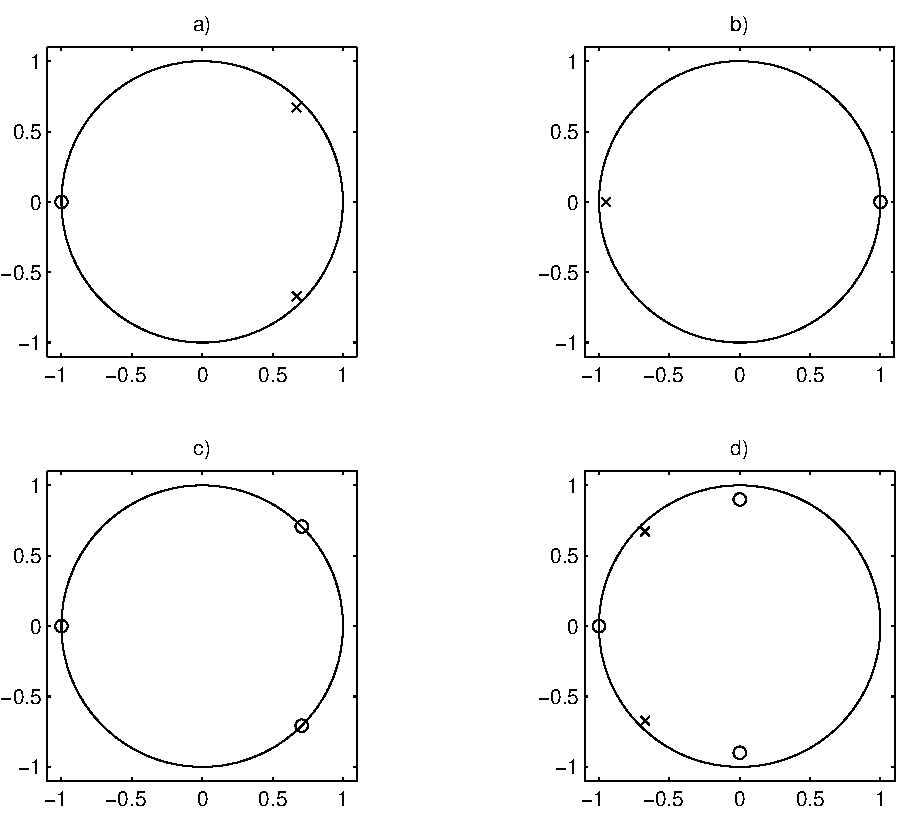
\includegraphics[width = 10cm]{psUeb/PolNullstellenUebung}
    \caption{\label{pic:SpektrenPolNullstellenplan} Verschiedene Systeme und ihre Pol- Nullstellenverteilung}
    \end{center}
    \end{figure}
    }
    \item Berechnen Sie das Spektrum einer Cosinus-Schwingung der Frequenz 2000 Hz bei einer
    Abtastrate von 6000 Hz, wenn Sie eine 6 Punkte DFT verwenden.
\end{enumerate}

\subsection{Aufgaben (Auf Klausurniveau)}
\begin{enumerate}
    \item Welche Pol-Nullstellenlage würde die folgende
    Betragsübertragungsfunktion mit dazugehöriger Phase bei einem reellwertigen, stabilen
    System zur Folge haben (fs = 8000 Hz)?
    (Genauere qualitative Skizze (Grosser Kreis bitte!)
    und kurze stichpunktartige Begründung für die relevanten Punkte)(8)
    \begin{figure}[H]
    \begin{center}
    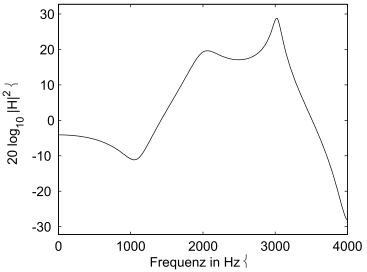
\includegraphics[width = 8cm]{psUeb/Betrag_14_20_18}
    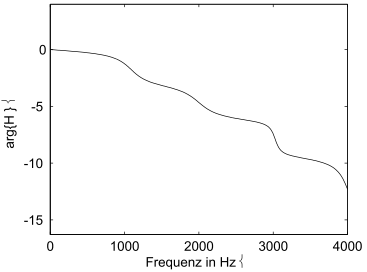
\includegraphics[width = 8cm]{psUeb/Phase_14_20_18}
    \end{center}
    \end{figure}

    \item Berechnen Sie die Übertragungsfunktion zur Impulsantwort $h(k) = [1\;\; 0\;\; 1]$
    \item Berechnen Sie die Übertragungsfunktion zu den folgenden Filtern. Skizzieren Sie
    die Funktion für $\alpha = 0.9$ und $\alpha = -0.9$
    \begin{enumerate}
        \item $y(k) = x(k) - \alpha y(k-1)$
    \end{enumerate}
    \item Ordnen Sie die folgenden Pol-Nullstellenpläne (a-d) den
        verschiedenen Übertragungsfunktionen (1-8) zu (2 Punkte für jede
        richtige Zuordnung, -1 Punkt für jede falsche).
        \begin{figure}[H]
        \begin{center}
        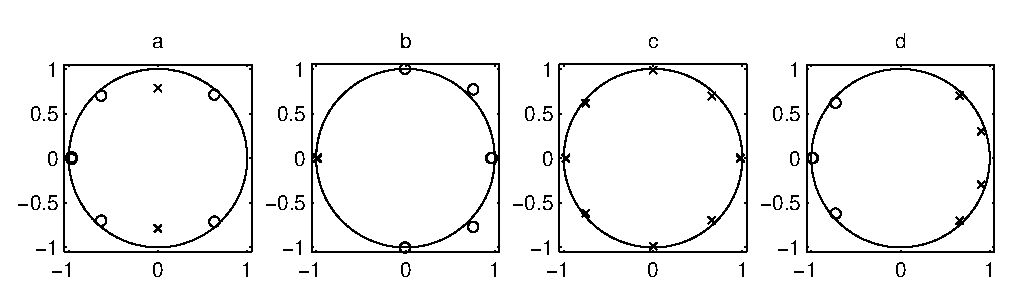
\includegraphics[width = 17cm]{psUeb/PolNullstellenKlausur2}
        \end{center}
        \end{figure}
        \begin{figure}[H]
        \begin{center}
        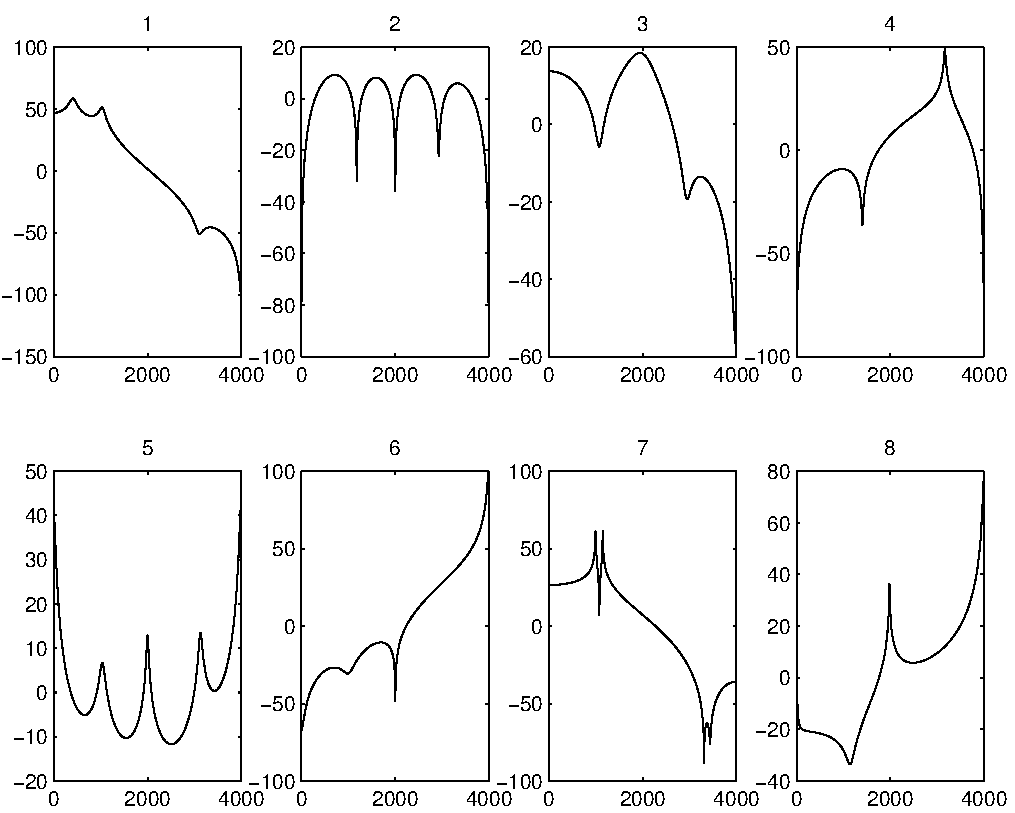
\includegraphics[width = 17cm]{psUeb/UebertragungKlausur2}
        \end{center}
        \end{figure}
    \item
\end{enumerate}

\compileif{bBook}
{
\subsection{Matlab-Aufgaben}
\begin{enumerate}
    \item Bestimmen Sie die Übertragungsfunktion der folgenden Systeme.
    \begin{enumerate}
        \item $y(k) = x(k) - \alpha y(k-1)$
        \item $y(k) =  0.3 x(k) + 07 x(k-1) + 1.9812 y(k-1)   - 1.0201 y(k-2)$
    \end{enumerate}
    \item
    \item
\end{enumerate}
}
\subsection{Transfer-Leistung}
\begin{enumerate}
    \item Bei der Berechnung des Faltungsprodukts muss bei der DFT/FFT auf
die Zirkularität geachtet werden. Welche Probleme können
auftreten, wenn das Ausgansspektrum nicht durch Multiplikation
$Y(n) = X(n)H(n)$, sondern durch eine Division $Y(n) = X(n)/H(n)$
entsteht (sog. Deconvolutionproblem)
    \item Welche Folge hat das Decimation in Time Prinzip der FFT für den Zusammenhang der
    Eingangsfolge zum berechneten Spektrum. Anders ausgedrückt, was ist notwendig, damit das Prinzip
    funktioniert.
    \item
\end{enumerate}
%
\compileif{bZusammenfassung}
{
\section{Zusammenfassung}
Die wichtigen Erkenntnisse aus diesem Kapitel sind:
\begin{itemize}
    \item LTI-Systeme erzeugen keine neuen Frequenzen.
    \item LTI-Systeme verändern nur den Betrag und Phase eines Signals. Die Betragsänderung
    über der Frequenz aufgetragen bezeichnet den Betragsfrequenzgang. Die Darstellung der Phase
    den Phasengang.
    \item Der Einfluss der Pole und Nullstellen lässt sich direkt am Einheitskreis ablesen.
    \item Stabile, kausale Systeme haben alle Pole innerhalb des Einheitskreises.
    \item Minimalphasige Systeme haben alle Nullstellen innerhalb des Einheitskreises.
    \item Die DTFT ist die z-Transformation für $z= e^{j\Omega}$.
    \item Die DFT ist eine zeitlich begrenzte DTFT, bei der das kontinuierliche Spektrum abgetastet wird.
    Sie ist deshalb maschinell berechenbar.
    \item Durch die Nutzung der DFT wird das Spektrum verändert.
    \begin{itemize}
        \item Das Zeitsignal wird als periodisch wiederholt angenommen
        \item Das Spektrum wird mit der Übertragungsfunktion des Fensters gefaltet. Es kommt zum
        sogenannten Leakage-Effekt.
    \end{itemize}
    \item Die Faltung lässt sich mit der DFT nur durch Zero-Padding realisieren.
    \item Reelle Signale haben ein konjugiert gerades Spektrum. Die Symmetrie ermöglicht eine
    Reduktion der Rechenleistung.
    \item Die Nutzung und Wahl der Fensterfunktionen zur Signalanalyse hängt im hohen Maße
    vom betrachteten Problem ab.
\end{itemize}
} 